% !TeX encoding = utf-8
% !TEX spellcheck = en-us
% !TeX program = pdflatex

% !Mode:: "TeX:UTF-8"
%%  本模板可以使用以下两种方式编译:
%%
%%     1. PDFLaTeX[推荐]
%%     2. XeLaTeX

%%  注意:
%%   1. 文件默认的编码为 UTF-8 对于windows,请选用支持UTF-8编码的编辑器。
%%   2. 若是模板有什么问题,请及时与我们取得联系,Email:latexstudio@qq.com。
%%   3. 可以到  https://ask.latexstudio.net 提问
 

\documentclass{swmcmthesis}

%%%%%%%%%%%%填写相关信息%%%%%%%%%%%%%%%%%%%%%%%%%%
\title{The \LaTeX{} Template  for swmcm} %论文题目

\baominghao{202200000001}           %报名号,修改为自己的队号

\zubie{ABCD} %选题

\abstract{ {\color{blue}This template was developed by \url{latexstudio.net}} (Your team's summary should be included as the first page of your electronic submission.) Type a summary of your results on this page. Do not include the name of your school, advisor, or team members on this page. \\ \centerline{
\includegraphics[width=.5\linewidth]{gongzhonghao-n}} \\ {\color{red}Papers must be submitted as an Adobe PDF electronic file, and typed in English, with a readable font of at least 12-point type. Be sure to change the control number and problem choice above.}}   % 摘要

\keywords{keyword1, keyword2, keyword3, keyword4}

\date{2022}

\begin{document}

% 生成首页
\maketitle
% 目录
\tableofcontents

\newpage

% -------------------------正文开始
\setcounter{page}{1}
\section{Introduction}
\lipsum[1]

\begin{center}
{{\Huge Please use pdflatex to compile this file}}
\end{center}

\subsection{Background}
\lipsum[1-2]

\subsection{Use figure}
\lipsum[1-2]

\begin{figure}[h!t]
	\centering
	
\includegraphics[width=0.6\textwidth]{example-image-a}
	\caption{caption}
	\label{fig:label}
\end{figure}

sub figure without title

\begin{figure}[h!t]
\centering
\subfigure{
\includegraphics[width=0.485\linewidth]{example-image-a}}\hfill
\subfigure{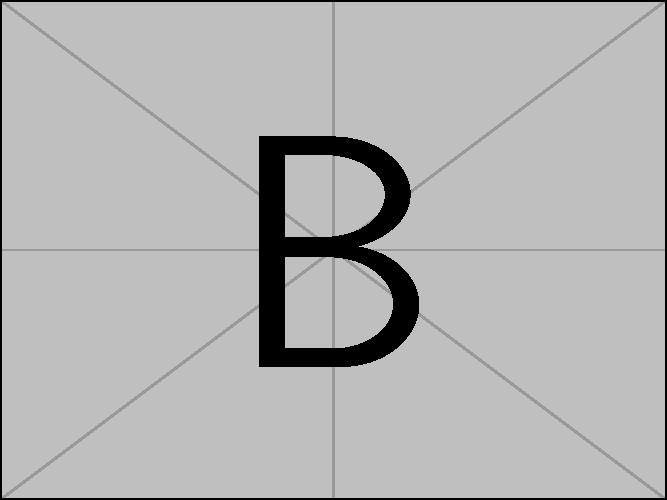
\includegraphics[width=0.485\linewidth]{example-image-b}}
\end{figure}

\newpage
sub figure with title

\begin{figure}[h!t]
\centering
\subfigure[title a]{
\includegraphics[width=0.485\linewidth]{example-image-a}}\hfill
\subfigure[title b]{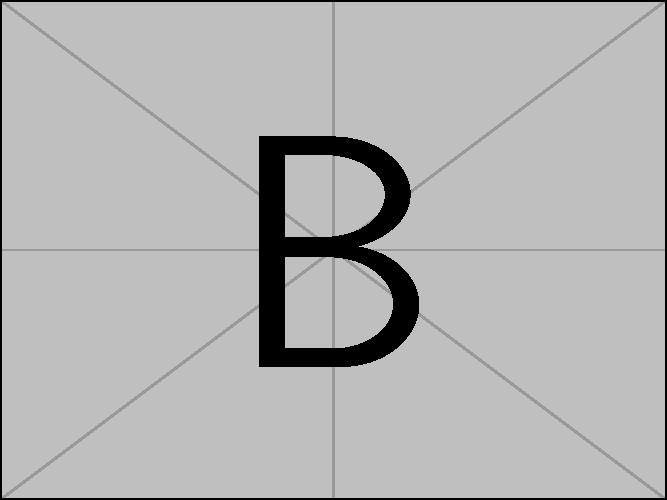
\includegraphics[width=0.485\linewidth]{example-image-b}}
\end{figure}

\section{Use table}

\begin{table}[h!t]
\centering
\caption{caption}
\label{tbl:label}
\begin{tabular}{cccccc}
\toprule
A & B & C & A & B & C \\
\midrule
12 & 23 & 34 & 12 & 23 & 34 \\
13 & 24 & 35 & 13 & 24 & 35 \\
14 & 25 & 36 & 14 & 25 & 36 \\
15 & 26 & 37 & 15 & 26 & 37 \\
\bottomrule
\end{tabular}
\end{table}

\subsection{Use Equation}

Eq.~\eqref{eq1} show the xxx
\begin{align}
\label{eq1}
a^2+b^2=c^2
\end{align}
where xxx

Eq.~\eqref{eq2} show the xxx
\begin{align}
\label{eq2}
a^2+b^2=c^2\\
\label{eq3}
a^2+b^2=c^2
\end{align}
where xxx

Eq.~\eqref{eq4} show the xxx
\begin{align}
\label{eq4}
\begin{cases}
a^2+b^2=c^2\\
a^2+b^2=c^2
\end{cases}
\end{align}
where xxx

\subsection{Use enumerate}

\begin{enumerate}
\item xxx
\item xxx
\item xxx
\item xxx
\end{enumerate}

\subsection{Analysis of question two}
\lipsum[1-2]

\section{Symbol and Assumptions}
\lipsum[1-2]

\subsection{Symbol Description}

\begin{table}[!h]
\centering
\begin{tabular}{cc}
\toprule[1.5pt]
Symbol & Description\\
\midrule[1pt]
$D$(in)  & xxx xxx\\
$P_u$(lbs)  & xxx xxx\\
$u_u$(in)  & xxx xxx\\
$\beta$  & xxx xxx\\
$G_f$(psi.in) & xxx xxx\\
\bottomrule[1.5pt]
\end{tabular}
\end{table}

\subsection{References cite}
Learn \LaTeX{} at Ref.\cite{bib:one}

Learn \LaTeX{} at Refs.\cite{bib:one,bib:two}

Learn \LaTeX{} at Refs.\cite{bib:one,bib:two,vedio,bib4}

\section{Model}
\lipsum[1-2]

\section{Test the Models}
\lipsum[1-2]

\section{Sensitivity Analysis}
\lipsum[1-2]

\section{Strengths and Weakness}
\lipsum[1-2]

\section{Conclusion}
\lipsum[1-2]

%----------------------------参考文献

\begin{thebibliography}{9}%宽度9
\bibitem{bib:one} \url{https://www.latexstudio.net}
\bibitem{bib:two} \url{https://wenda.latexstudio.net}
\bibitem{vedio} \url{https://space.bilibili.com/209746320}

\bibitem{bib4} L. Prandtl, Fluid motions with very small friction, Proceedings of the 3rd International Mathematical Congress, Heidelberg: H. Schlichting, 1904, 484-491.

\bibitem{bib5} K. O. Friedriehs and W. Wasow, Singular perturbations of nonlinear oscillations, Duke. Math. J., 1946, 13: 367-381.

\bibitem{bib6} W. Wasow, Asymptotic Expansions for Ordinary Differential Equations, Interscience, New York, 1965.
\end{thebibliography}

% ---------------------开始附录

\newpage

\section*{Appendix}
% 在目录中添加Appendix
\addcontentsline{toc}{section}{Appendix}

\begin{lstlisting}[language=matlab,caption={The matlab Source code of Algorithm}]
kk=2;[mdd,ndd]=size(dd);
while ~isempty(V)
[tmpd,j]=min(W(i,V));tmpj=V(j);
for k=2:ndd
[tmp1,jj]=min(dd(1,k)+W(dd(2,k),V));
tmp2=V(jj);tt(k-1,:)=[tmp1,tmp2,jj];
end
tmp=[tmpd,tmpj,j;tt];[tmp3,tmp4]=min(tmp(:,1));
if tmp3==tmpd, ss(1:2,kk)=[i;tmp(tmp4,2)];
else,tmp5=find(ss(:,tmp4)~=0);tmp6=length(tmp5);
if dd(2,tmp4)==ss(tmp6,tmp4)
ss(1:tmp6+1,kk)=[ss(tmp5,tmp4);tmp(tmp4,2)];
else, ss(1:3,kk)=[i;dd(2,tmp4);tmp(tmp4,2)];
end;end
dd=[dd,[tmp3;tmp(tmp4,2)]];V(tmp(tmp4,3))=[];
[mdd,ndd]=size(dd);kk=kk+1;
end; S=ss; D=dd(1,:);
 \end{lstlisting}
\begin{lstlisting}[language=c,caption={The lingo source code}]
kk=2;
[mdd,ndd]=size(dd);
while ~isempty(V)
    [tmpd,j]=min(W(i,V));tmpj=V(j);
for k=2:ndd
    [tmp1,jj]=min(dd(1,k)+W(dd(2,k),V));
    tmp2=V(jj);tt(k-1,:)=[tmp1,tmp2,jj];
end
    tmp=[tmpd,tmpj,j;tt];[tmp3,tmp4]=min(tmp(:,1));
if tmp3==tmpd, ss(1:2,kk)=[i;tmp(tmp4,2)];
else,tmp5=find(ss(:,tmp4)~=0);tmp6=length(tmp5);
if dd(2,tmp4)==ss(tmp6,tmp4)
    ss(1:tmp6+1,kk)=[ss(tmp5,tmp4);tmp(tmp4,2)];
else, ss(1:3,kk)=[i;dd(2,tmp4);tmp(tmp4,2)];
end;
end
    dd=[dd,[tmp3;tmp(tmp4,2)]];V(tmp(tmp4,3))=[];
    [mdd,ndd]=size(dd);
    kk=kk+1;
end;
S=ss;
D=dd(1,:);
 \end{lstlisting}

% ----------------
% 在目录中添加格式规范,可以删掉

% \section*{Format specification}
\addcontentsline{toc}{section}{Format specification}

\includepdfmerge{shuwei,1-2}

\end{document} 